\chapter{Vulnerabilità sfruttabili dalla ROP e difese}
\label{chap:ROP-vulnerabilities}

\section{Vulnerabilità critiche all'interno dei codici}
\label{sec:Vulnerabilita}
Nel capitolo \ref{chap:ROP} sono stati ampiamente discussi i punti fondamentali su cui si basa la \textbf{ROP}. Tuttavia, non è ancora stato approfondito in quali condizioni sia possibile applicare questa tecnica di attacco in un
vero e proprio software. Effettuare un attacco con essa, significa sovvertire il controllo del flusso dell'applicazione in modo tale che vengano eseguite le azioni richieste dall'utente malevolo. Una delle classi di vulnerabilità
più conosciute e diffuse al mondo che consentono di svolgere quanto appena descritto, è la \textit{stack-based buffer overflow} \cite*{Stack-bufferoverflow}\cite*{Stack-bufferoverflow2}. Esistono altre classi della stessa tipologia, quali: \textit{heap overflow} 
\cite*{Heapoverflow}\cite*{Heapoverflow-jpeg}, \textit{integer overflow} \cite*{Integeroverflow}\cite*{Integeroverflow2} e \textit{format string vulnerabilities} \cite*{Formatstring}\cite*{Formatstring2}.\\
In questo elaborato saranno approfonditi solo gli \textit{stack-based buffer overflow} e le \textit{format string vulnerabilities}, in quanto saranno le due tipologie presenti anche all'interno dei test.

\subsection{Stack-based buffer overflow}
\label{subsec:Stack-buffer overflow}
Nelle precedenti sezioni è stato assunto che fosse possibile sovrascrivere l'indirizzo di ritorno memorizzato nello stack di un codice scritto in linguaggio C, consentendo ad un attaccante di applicare la \textbf{ROP}. 
Tuttavia, non è ancora stato chiarito come sia possibile o quali siano le condizioni che consentano di effettuare questa operazione. Solitamente, un utente qualsiasi non dovrebbe essere in grado di modificare aree 
di memoria sensibili (come lo stack) riservate ad un programma in esecuzione. Esistono però delle vulnerabilità che se sfruttate correttamente ne conferiscono all'attaccante il controllo, rendendo di fatto possibili exploit 
come quelli di tipo \textbf{Return Oriented Programming}.\\
Una delle classi di vulnerabilità più conosciute e diffuse nel mondo della programmazione, che porta a questo tipo di conseguenze, è la \textit{stack-based buffer overflow}. Come espresso nella sezione \ref{subsec:stack} del capitolo \ref*{chap:ROP}, nel frame stack
attuale vengono salvati dati come variabili locali, argomenti passati alla funzione e indirizzo di ritorno. Il problema sorge quando all'interno di una subroutine viene definito un buffer, ossia viene riservata una sequenza di lunghezza predefinita di celle o blocchi di
memoria (lo si può anche pensare semplicemente come un qualsiasi array). Essendo esso una qualsiasi variabile, il suo contenuto verrà di conseguenza memorizzato nello stack frame corrispondente. Tuttavia, se per l'utente fosse possibile inserire più dati all'interno di questo buffer,
rispetto allo spazio riservato in precedenza dal programma, allora si verificherebbe quello che viene comunemente definito come \textit{buffer overflow} \cite*{Stack-bufferoverflow}.\\
Grazie a questo fenomeno, l'attaccante potrà quindi sovrascrivere il contenuto dell'attuale stack frame con codice arbitrario, prendendo di fatto pieno controllo del flusso del programma. Nel caso della ROP, l'utente malintenzionato avrà come scopo quello di identificare la 
posizione nella quale è stato memorizzato l'indirizzo di ritorno nello stack, per poterlo sovrascrivere con un altro indirizzo effettuando un dirottamento del normale flusso d'esecuzione previsto dal programmatore \cite*{ROP-bufferoverflow}.

\begin{figure}[htpb]
    \centerline{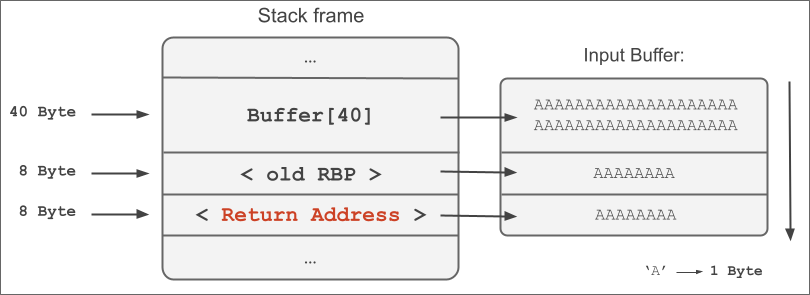
\includegraphics[scale=.6]{images/stack-based buffer overflow.png}}
    \caption{Esempio di sovrascrittura dopo 48 Byte dell'indirizzo di ritorno nello stack frame tramite input inserito in Buffer (56 'A' inserite in Buffer).}
    \label{fig:Stack-overflow}
\end{figure}

Esistono diverse funzioni ``insicure'' nel linguaggio di programmazione \textbf{C} che se non gestite in maniera accurata possono portare a vulnerabilità di questo tipo, alcune di queste sono ad esempio la \textit{gets}, la \textit{strcpy} \cite*{unsafe-func} e se non utilizzata in maniera opportuna 
anche la \textbf{read}. La prima delle tre non limita in alcun modo l'input che sarà inserito dall'utente, conferendo la possibilità di introdurre qualsiasi dato nello stack. La seconda funzione invece copia il contenuto della seconda stringa nella prima stringa specificata 
(ogni sequenza di caratteri in C è un buffer), ed anche in questo caso la copia sarà effettuata senza nessun controllo sulle dimensioni dei due buffer. L'ultimo caso prevede che sia l'utente a specificare il numero massimo di dati inseribili, tuttavia se questo dato fosse impostato in 
maniera scorretta un eventuale attaccante avrebbe la possibilità di oltrepassare l'area riservata al buffer sovrascrivendo il contenuto dello stack.\\
Allo stato attuale alcune delle funzioni considerate ``insicure'' sono state sostituite con altre versioni delle stesse più affidabili, come \textit{fgets} e \textit{snprintf} rispettivamente per \textit{gets} e \textit{strcpy} \cite*{unsafe-func}.\\
Una volta chiarita la principale vulnerabilità, la quale verrà sfruttata durante la fase dei test, un'altra classe sempre molto importante e pericolosa verrà approfondita, ossia le \textit{format string vulnerabilities}.

\subsection{Format string}
\label{subsec:format string}
Questa classe di vulnerabilità prende il suo nome dalla tipologia di argomento che può essere passato ad una \textit{format function}, uno speciale tipo di funzione ANSI C, quale \textbf{printf}, \textbf{scanf} o un'altra della stessa categoria. Questa tipologia di funzione può prendere un numero variabile di
argomenti, tra i quali appunto le \textit{format strings}, e sono utilizzate per convertire un tipo di dato semplice nella sua rappresentazione in stinga \cite*{Formatstring}.\\ 
Una \textit{format string} è una stringa contenente testo e delle direttive di formato, quindi delle specifiche utili al compilatore per apprendere correttamente il tipo di una variabile. Esistono molteplici tipologie di queste speciali direttive, questo per fornire una rappresentazione corretta per ogni tipo di
dato fornito. Alcune di queste sono: 

\begin{table}[h]
    \centering
    \begin{tabular}{ |c|p{6cm}|  }
        \hline
        \textbf{Tipologia} & \textbf{Scopo} \\
        \hline
        ``\%d'' & stampare degli interi \\
        ``\%s'' & stampare una stringa \\
        ``\%p'' & stampare il valore di un puntatore \\
        ``\%x'' & stampare caratteri esadecimali \\
        \hline
    \end{tabular}
\end{table}

Queste direttive, infatti, sono inizialmente \textbf{interpretate} e successivamente \textbf{sostituite} con il valore appropriato. Ad esempio, in un'ipotetica chiamata alla funzione \textbf{printf}, se il primo argomento passato sarà una \textit{format string}, essa verrà rimpiazzata col valore effettivo
della variabile passata come secondo argomento (sempre che sia compatibile col tipo di variabile inserito), ed infine stampata.

\begin{figure}[htpb]
    \centerline{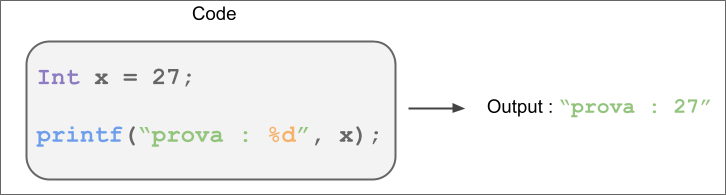
\includegraphics[scale=.5]{images/format string.png}}
    \caption{Esempio di printf con direttiva di formato ``\%d'' nel primo argomento e variabile di tipo intero come secondo.}
    \label{fig:format string}
\end{figure}

Tuttavia, se come chiamata verrà effettuata la seguente: \textbf{printf}(\textit{str}), dove \textit{str} può essere una \textit{format string} contenente più direttive di formato, come la seguente: ``\%x\%x''. L'output che ne risulterà sarà il contenuto dei registri \textbf{rsi} e \textbf{rdx} in esadecimale. Aggiungendo ulteriori direttive è possibile recuperare i dati 
memorizzati nello stack, reperendo molte informazioni sensibili che non sarebbero altrimenti accessibili. La causa per cui questo accade è per via dalle \textbf{convinzioni di chiamata}\label{call-convention} definite nel set di specifiche \textbf{System V AMD64 ABI} \cite*{AMD64-ABI} (utilizzate dall'architettura x86-64). Esse prevedono che per ogni chiamata 
a funzione i primi sei argomenti siano memorizzati nei registri \textbf{rdi}, \textbf{rsi}, \textbf{rdx}, \textbf{rcx}, \textbf{r8}, \textbf{r9}, mentre gli eventuali restanti verranno caricati nello stack. Quest'ultimo punto è quello che rende possibile la lettura dei dati contenuti nello stack mediante le \textit{format strings}. La \textit{format function}
cercherà di reperire ciò che l'utente vuole stampare dallo stack, fornendogli qualsiasi dato presente in esso.\\
Essendo questa una delle vulnerabilità più pericolose e frequenti intorno agli anni 2000 \cite*{Formatstring}, col passare del tempo sono state trovate delle soluzioni a tale problema. Anche se molte di esse prevedono sempre che vi sia particolare attenzione da parte del programmatore durante la stesura del codice.
Attualmente, i moderni compilatori evidenziano errori quando l'utente sta cercando di compilare del codice contenente una \textit{format function} mal gestita \footnote[1]{Un esempio di format function mal gestita può essere quella vista in precedenza, ossia \textbf{printf}(\textit{str}).}, invitandolo a modificarla per renderla più sicura.
Esistono altrimenti delle regole applicabili al proprio codice definite nel \textbf{SEI CERT C Coding Standard}, che permettono di rendere più sicure le applicazioni sviluppate \cite*{SEI-CERT-RULE09}.

\section{Difese superabili dalla ROP}
\label{sec:Def-bypass}
Nella sezione \ref{sec:Vulnerabilita} sono state approfondite alcune delle principali vulnerabilità che possono portare ad un exploit di un programma mediante la \textbf{ROP}. Ora ci si concentrerà nell'evidenziare quali difese questa potente tecnica è in grado di eludere e quali invece risultino particolarmente efficaci contro di essa.\\
Le principali difese che la ROP è in grado di superare abilmente sono: \textbf{W$\oplus$X} (\textbf{Write  xor Execute}) e \textbf{ASLR} (\textbf{Address Space Layout Randomization}).

\subsection{W$\oplus$X (W-xor-X)}
\label{sec:Def-W-xor-X}
\textbf{W$\oplus$X} o meglio conosciuta come \textbf{W-xor-X}, è un meccanismo di difesa introdotta per la prima volta nel sistema \textbf{OpenBSD}\footnote[2]{\textbf{OpenBSD} è un sistema \textit{unix-like}, open-source e basato principalmente sulla sicurezza.} nel 2003 \cite*{OpenBSD-3.3}. Col passare degli anni venne introdotto anche negli altri sistemi 
assumendo diversi nomi come \textbf{DEP} (\textbf{Data Execution Prevention})\cite*{DEP-windows}, e direttamente all'interno dei processori col nome di \textbf{NX bit} (\textbf{No-execute})\cite*{NX}.\\
Il suo compito è quello di rendere non eseguibili specifiche aree di memoria, cosicché eventuali tentativi di eseguire codice macchina in quelle aree causeranno un'eccezione. Questa tecnica venne introdotta anche per evitare gli attacchi shellcode \cite*{shellcode}\cite*{Stack-bufferoverflow}, i quali sfruttavano vulnerabilità per ottenere il controllo del flusso
del programma ed iniettavano il codice macchina per invocare una \textit{shell} direttamente dallo stack. Rendendo queste aree di memoria non eseguibile è possibile evitare tale tipologia di attacchi. Nonostante non sia abbastanza efficace da bloccare la \textbf{ROP}, che a differenza delle shellcode non inietterà nuovo codice da eseguire \cite*{ASLR-WX}, ma sfrutterà i \textbf{gadgets} già presenti nei file.\\

\subsection{ASLR (Address Space Layout Randomization)}
\label{sec:Def-ASLR}
\textbf{ASLR} (\textbf{Address Space Layout Randomization}) \cite*{ASLR}\Cite*{ASLR-WX} è una tecnica di sicurezza, che venne per la prima volta implementata nei sistemi operativi nel 2001. Come la \textbf{W$\oplus$X}, ha lo scopo di prevenire l'exploit di eventuali vulnerabilità che possono consentire ad un attaccante di corrompere aree di memoria.\\
Questa meccanica di difesa consiste nel rendere (parzialmente) casuale l'indirizzo su cui risiedono le funzioni di libreria e delle più importanti aree di memoria associate ad un programma in esecuzione. In questo modo, un attaccante non sarà in grado di reperire gli indirizzi necessari per eseguire codice malevolo prima che il programma sia effettivamente eseguito.\\
Come si vedrà nelle sezioni successive di questo elaborato, esistono più metodi utilizzando la \textbf{ROP} per bypassare tale tipologia di difesa.
